\documentclass[14pt,aspectratio=169]{beamer}

\usepackage{amssymb, amsmath}
%\usepackage[all]{xy}

\usepackage{alltt}
\usepackage{pslatex}
\usepackage{epigraph}
\usepackage{verbatim}

\usepackage{url}

%\usepackage{graphicx}
\usepackage{latexsym}
\usepackage{array}
\usepackage{comment}
\usepackage{makeidx}
\usepackage{listings}
\usepackage{indentfirst}
\usepackage{verbatim}
\usepackage{color}
\usepackage{url}
\usepackage{xspace}
%\usepackage{fontspec}
%\usepackage{xunicode}
%\usepackage{xltxtra}
%\usepackage{xecyr}
\usepackage{hyperref}
%\usepackage[english]{babel}
%\usepackage[utf8]{inputenc}
%\setmainfont[Mapping=tex-text]{DejaVu Serif}
%\setsansfont[Mapping=tex-text]{DejaVu Sans}
%\setmonofont[Mapping=tex-text]{DejaVu Sans Mono}
%\usepackage{polyglossia}
%\setdefaultlanguage{russian}
\usepackage{stmaryrd}

\usepackage{amsmath, amsthm, amssymb}
\usepackage{graphicx}
\usepackage{euscript}
\usepackage{mathtools}
\usepackage{xcolor}
\usepackage{multirow}
\usepackage{pgfplots}

\makeatletter
\begin{comment}
\newcolumntype{e}[1]{%--- Enumerated cells ---
   >{\minipage[t]{\linewidth}%
     \NoHyper%                Hyperref adds a vertical space
     \let\\\tabularnewline
     \enumerate
        \addtolength{\rightskip}{0pt plus 50pt}% for raggedright
        \setlength{\itemsep}{-\parsep}}%
   p{#1}%
   <{\@finalstrut\@arstrutbox\endenumerate
     \endNoHyper
     \endminipage}}

\newcolumntype{i}[1]{%--- Itemized cells ---
   >{\minipage[t]{\linewidth}%
        \let\\\tabularnewline
        \itemize
           \addtolength{\rightskip}{0pt plus 50pt}%
           \setlength{\itemsep}{-\parsep}}%
   p{#1}%
   <{\@finalstrut\@arstrutbox\enditemize\endminipage}}

\AtBeginDocument{%
    \@ifpackageloaded{hyperref}{}%
        {\let\NoHyper\relax\let\endNoHyper\relax}}
\end{comment}

\makeatother

\definecolor{shadecolor}{gray}{1.00}
\definecolor{darkgray}{gray}{0.30}

\newcommand{\set}[1]{\{#1\}}
\newcommand{\angled}[1]{\langle {#1} \rangle}
\newcommand{\fib}{\rightarrow_{\mathit{fib}}}
\newcommand{\fibm}{\Rightarrow_{\mathit{fib}}}
\newcommand{\oo}[1]{${#1}^o$}
\newcommand{\inml}[1]{\mbox{\lstinline{#1}}}
\newcommand{\goal}{\mathfrak G}
\newcommand{\inmath}[1]{\mbox{$#1$}}
\newcommand{\sembr}[1]{\llbracket{#1}\rrbracket}

\newcommand{\withenv}[2]{{#1}\vdash{#2}}
\newcommand{\ruleno}[1]{\mbox{[\textsc{#1}]}}
\newcommand{\trule}[2]{\dfrac{#1}{#2}}

%\setlength{\epigraphwidth}{.55\textwidth}

\definecolor{light-gray}{gray}{0.90}
\newcommand{\graybox}[1]{\colorbox{light-gray}{#1}}

\newcommand{\nredrule}[3]{
  \begin{array}{cl}
    \textsf{[{#1}]}& 
    \begin{array}{c}
      #2 \\
      \hline
      \raisebox{-1pt}{\ensuremath{#3}}
    \end{array}
  \end{array}}

\newcommand{\naxiom}[2]{
  \begin{array}{cl}
    \textsf{[{#1}]} & \raisebox{-1pt}{\ensuremath{#2}}
  \end{array}}

\lstdefinelanguage{ocaml}{
keywords={let, begin, end, in, match, type, and, fun, 
function, try, with, class, object, method, of, rec, until,
while, not, do, done, as, val, inherit, module, sig, @type, struct, 
if, then, else, open, virtual, new, fresh, conde, run},
sensitive=true,
basicstyle=\small,
commentstyle=\scriptsize\rmfamily,
keywordstyle=\ttfamily\bfseries,
identifierstyle=\ttfamily,
basewidth={0.5em,0.5em},
columns=fixed,
fontadjust=true,
moredelim=**[is][\color{red}]{@}{@},
literate={fun}{{$\lambda$}}1 {->}{{$\to$}}3 {===}{{$\equiv$}}1 {=/=}{{$\not\equiv$}}1 {|>}{{$\triangleright$}}3 {\&\&\&}{{$\wedge$}}2 {|||}{{$\vee$}}2 {^}{{$\uparrow$}}1,
morecomment=[s]{(*}{*)}
}

\lstset{
mathescape=true,
basicstyle=\small,
identifierstyle=\ttfamily,
keywordstyle=\bfseries,
commentstyle=\scriptsize\rmfamily,
basewidth={0.5em,0.5em},
fontadjust=true,
escapechar=!,
language=ocaml
}

\begin{comment}
\lstdefinelanguage{ocaml}{
keywords={fresh, let, begin, end, in, match, type, and, fun, function, try, with, when, class,
object, method, of, rec, until, while, not, do, done, as, val, inherit,
new, module, sig, deriving, datatype, struct, if, then, else, open, private, virtual, include, @type},
sensitive=true,
commentstyle=\small\itshape\ttfamily,
keywordstyle=\ttfamily\underbar,
identifierstyle=\ttfamily,
basewidth={0.5em,0.5em},
columns=fixed,
fontadjust=true,

literate={->}{{$\to\;\;$}}3 {===}{{$\equiv$}}3 {=/=}{{$\not\equiv$}}3 {|>}{{$\triangleright$}}3,
morecomment=[s]{(*}{*)}
}

\lstset{
mathescape=true,
identifierstyle=\ttfamily,
keywordstyle=\bfseries,
commentstyle=\scriptsize\rmfamily,
basewidth={0.5em,0.5em},
fontadjust=true,
language=ocaml
}
\end{comment}
\sloppy

\newcommand{\miniKanren}{\texttt{miniKanren}\xspace}
\newcommand{\ocanren}{\texttt{OCanren}\xspace}
\newcommand{\ocaml}{\texttt{OCaml}\xspace}
\newcommand{\mk}{\texttt{miniKanren}\xspace}
\newcommand{\inbr}[1]{\langle #1 \rangle}
\renewcommand{\emptyset}{\varnothing}

\definecolor{myRed}{rgb}{0.6, 0, 0}

\setbeamertemplate{footline}[frame number]
\setbeamertemplate{navigation symbols}{}
\setbeamertemplate{blocks}[rounded][shadow=true] 
\beamertemplateballitem

\mode<presentation>{
  \usetheme{default}
}

\theoremstyle{definition}

\title{On Fair Conjunction 
}


\author{
 \underline{Petr Lozov} \and Dmitry Boulytchev
}

\institute[]{
\small{
\textbf{Saint Petersburg State University $\: $\\JetBrains Research}
}
}

\date{
   \vskip 1cm
   \small{
   \textbf{miniKanren workshop}\\
   August 27, 2020\
  }
}

\begin{document}

\begin{frame}[plain]
  \titlepage
\end{frame}

\begin{frame}[fragile]{Conjunction in ~\mk}
Operation to find common answers for several goals
\vskip5mm
\begin{itemize}
  \item[$\bullet$] Asymmetrical operation
  \vskip2mm
  \item[$\bullet$] Order of conjuncts affects 
  \begin{itemize}
    \normalsize	
    \item[$\circ$] Performance
    \pause
    \item[$\circ$] \textbf{Convergence}
  \end{itemize}
\end{itemize}
\end{frame}

\begin{frame}[fragile]{Conjunction Example (1/2)}
\begin{center}
\begin{tabular}{c}
\begin{lstlisting}
let reverse$^o$ x y = conde [ 
  x === [] &&& y === []; 
  fresh (a xs ys) 
    (x === a :: xs)
    (append$^o$ ys [a] y)
    (reverse$^o$ xs ys)
\end{lstlisting} \\
\end{tabular}
\end{center}
\vskip1cm
\pause
\begin{center}
\begin{tabular}{c}
\begin{lstlisting}
     run$^*$ q (reverse$^o$ [1;2;3] q) $\rightarrow$ [ [3;2;1], ...
$\pause$
     run$^*$ q (reverse$^o$ q [1;2;3]) $\rightarrow$ [ [3;2;1] ]
\end{lstlisting}
\end{tabular}
\end{center}

\end{frame}

\begin{frame}[fragile]{Conjunction Example (2/2)}
\begin{center}
\begin{tabular}{c}
\begin{lstlisting}
let reverse$^o$ x y = conde [ 
  x === [] &&& y === []; 
  fresh (a xs ys) 
    (x === a :: xs)
    (reverse$^o$ xs ys)
    (append$^o$ ys [a] y)
\end{lstlisting} \\
\end{tabular}
\end{center}
\vskip1cm
\pause
\begin{center}
\begin{tabular}{c}
\begin{lstlisting}
     run$^*$ q (reverse$^o$ [1;2;3] q) $\rightarrow$ [ [3;2;1] ]
$\pause$
     run$^*$ q (reverse$^o$ q [1;2;3]) $\rightarrow$ [ [3;2;1], ...
\end{lstlisting}
\end{tabular}
\end{center}

\end{frame}

\begin{frame}[fragile]{Fair Conjunction}
\centering

$g_1 \; \land \; g_2$ converges $\;\Leftrightarrow\;$ $g_2 \; \land \; g_1$ converges

\vskip1cm
\textbf{Goal} \\
Introduce fair conjunction into the \mk

\end{frame}

\begin{frame}{Talk Outline}

\begin{enumerate}
  \item Semantics of directed conjunction
  \vskip6mm
  \item Semantics of naive fair conjunction
  \vskip6mm
  \item Semantics of fair conjunction by structural recursion
\end{enumerate}

\end{frame}

\begin{frame}[fragile]{Semantics of Directed Conjunction}
\begin{itemize}
    \item[$\bullet$] Described as a \emph{deterministic Labeled Transition System}
    \item[$\bullet$] Supports interleaving of clauses
    \item[$\bullet$] The state uniformly stores all conjuncts
    \item[$\bullet$] Minimum step is unfolding of one relational call
\end{itemize}
\end{frame}

\begin{frame}[fragile]{Some Definitions}
\textbf{States:}
\[
\begin{array}{rcll}
  c & = & F\,(t_1,\dots,t_k) & \mbox{relational call} \\
  T & = & T \lor T & \mbox{disjunction state} \\
               & \mid & \inbr{\sigma;\, c_1 \land \dots \land c_n} & \mbox{leaf state}\\[2mm]
T & +=& \emptyset & \mbox{empty state}
\end{array}
\]

\textbf{Transitions:}
\[
\begin{array}{cl}
T \xrightarrow{\circ} T  & \mbox{step without answer} \\
T \xrightarrow{\sigma} T & \mbox{step with answer } \sigma
\end{array}
\]
\end{frame}

\begin{frame}[fragile]{Unfolding}
$unfold(\sigma, F\,(t_1,\dots,t_k)) = T$
\vskip1cm

Unfolding steps:
\begin{enumerate}
    \item Replace $F$ by body of relation $F$
    \item Substitute arguments $t_1,\dots,t_k$ to the body
    \item Evaluate all fresh variable introductions and unifications using substitution $\sigma$ 
    \item Reduce to disjunctive normal form and represent as a state
\end{enumerate}

\end{frame}

\begin{frame}[fragile]{Unfolding: Example}
  \begin{center}
  \begin{tabular}{c}
\begin{lstlisting}
let reverse$^o$ x y = conde [ 
  x === [] &&& y === []; 
  fresh (a xs ys) 
    (x === a :: xs)
    (reverse$^o$ xs ys)
    (append$^o$ ys [a] y)
\end{lstlisting} \\
\end{tabular}
\vskip1cm
\begin{tabular}{rcll}
  $unfold(\set{},$ \lstinline|reverse$^o$ $\alpha$ []| $)$ & = & 
  $\inbr{\set{\alpha = \lstinline|[]|}; \epsilon}$ \\
  & $\lor$ & $\langle\set{\alpha = \alpha_1 \lstinline|::| \alpha_2};$ & \lstinline|reverse$^o$ $\alpha_2$ $\alpha_3$| $\land$ \\
  & & & \lstinline|append$^o$ $\alpha_3$ [$\alpha_1$] []|$\rangle$
\end{tabular}
  \end{center}
\end{frame}

\begin{frame}[fragile]{Semantics of Directed Conjunction (1/2)}
\[\begin{array}{cr}
     {\inbr{\sigma;\, \epsilon} \xrightarrow{\sigma} \emptyset}  
&     \ruleno{Answer} \\[4mm]
\dfrac{T_1 \xrightarrow{\alpha} \emptyset}
      {T_1 \lor T_2 \xrightarrow{\alpha} T_2}
&     \ruleno{Disj} \\[8mm]
\dfrac{T_1 \xrightarrow{\alpha} \bar{T_1} \qquad \bar{T_1} \not= \emptyset}
      {T_1 \lor T_2 \xrightarrow{\alpha} T_2 \lor\bar{T_1}}
&     \ruleno{DisjStep}
\end{array}\]
\end{frame}

\begin{frame}[fragile]{Semantics of directed conjunction (2/2)}

\begin{center}
    Directed conjunction always evaluates the first conjunct 
\end{center}

\[\begin{array}{cr}
\dfrac{unfold(\sigma, c) = T}
      {\inbr{\sigma;\, c \land C} \xrightarrow{\circ} push(\Box \land C, T)}
&     \ruleno{ConjUnfold}
\end{array}\]
\end{frame}

\begin{frame}[fragile]{Naive Fair Conjunction}
\begin{itemize}
    \item[$\bullet$] \emph{Unfolding bound} $\textcolor{myRed}{N}$ is global parameter of semantics
    \item[$\bullet$] Conjuncts unfold from left to right
    \item[$\bullet$] Each conjunt unfolds no more than $\textcolor{myRed}{N}$ times
    \item[$\bullet$] If all conjuncts are unfolded $\textcolor{myRed}{N}$ times, then again go to the leftmost conjunct
\end{itemize}
\end{frame}

\begin{frame}[fragile]{Updated States}

\[
\begin{array}{rcll}
  c & = & F^{\textcolor{myRed}{k}}\,(t_1,\dots,t_k) & \mbox{relational \underline{marked} call} \\
  T & = & T \lor T & \mbox{disjunction state} \\
               & \mid & \inbr{\sigma;\, c_1 \land \dots \land c_n} & \mbox{leaf state}\\[2mm]
T & +=& \emptyset & \mbox{empty state}
\end{array}
\]

\end{frame}

\begin{frame}[fragile]{Semantics of Naive Fair Conjunction}

\begin{center}
    Naive fair conjunction unfolds each conjunct $N$ times
\end{center}

\[\begin{array}{cr}
      {\inbr{\sigma;\, c_1^0 \land \ldots \land c_n^0} \xrightarrow{\circ} (\sigma, i, c_1^N \land \ldots \land c_n^N)}
&     \ruleno{ConjZero} \\[8mm]
\dfrac{\begin{array}{c}
      c_k^m \mbox{ is the first conjunct with } m > 0 \\ 
      unfold(\sigma, c_k) = T \qquad set(T, m - 1) = \bar{T}
      \end{array}}
      {
      \inbr{\sigma;\, C_1 \land c_k^m \land C_2} \xrightarrow{\circ} push(C_1 \land \Box \land C_2, \bar{T})
      }
&     \ruleno{ConjUnfold}
\end{array}\]
\end{frame}

\begin{frame}[fragile]{Naive Fair Conjunction: Example}
\begin{center}
\begin{tabular}{m{15em}c}
\begin{lstlisting}
let rec repeat e l =
  (l === []) |||
  (fresh (ls)
    (l === e : ls)
    (repeat e ls))
\end{lstlisting} &
\begin{lstlisting}
let divergence l = 
  repeat C$_1$ l &&& 
  repeat C$_2$ l
$\,$
$\,$
$\,$
\end{lstlisting}
\end{tabular}

\begin{tabular}{rl}
                      & 
\lstinline|$\langle\set{}$; divergence$^2$ $\alpha_0\rangle$| \\ \pause
$\xrightarrow{\circ}\!\!\!\!$ &
\lstinline|$\langle\set{}$; repeat$^1$ C$_1$ $\alpha_0$ $\land$ repeat$^1$ C$_2$ $\alpha_0\rangle$| \\ \pause
$\xrightarrow{\circ}\!\!\!\!$ &
\lstinline|$\langle\{\alpha_0 =$ []$\}$; repeat$^1$ C$_2$ $\alpha_0\rangle$ $\lor$ $\langle\{\alpha_0 =$ C$_1$:$\,\alpha_1\}$; repeat$^0$ C$_1$ $\alpha_1$ $\land$ repeat$^1$ C$_2$ $\alpha_0\rangle$| \\ \pause
$\xrightarrow{\circ}\!\!\!\!$ &
\lstinline|$\langle\{\alpha_0 =$ C$_1$:$\,\alpha_1\}$; repeat$^0$ C$_1$ $\alpha_1$ $\land$ repeat$^1$ C$_2$ $\alpha_0\rangle$ $\lor$ $\langle\{\alpha_0 =$ []$\}$; $\epsilon\rangle$| \\ \pause
$\xrightarrow{\circ}\!\!\!\!$ &
\lstinline|$\langle\{\alpha_0 =$ []$\}$; $\epsilon\rangle$| $\xrightarrow{\{\alpha_0 = []\}} \emptyset$ \\
\end{tabular}
\end{center}
\end{frame}

\begin{frame}[fragile]{Drawbacks of Naive Fair Conjunction}
\begin{itemize}
    \item[$\bullet$] \emph{Unfolding bound} $\textcolor{myRed}{N}$ is global parameter of semantics
    \vskip5mm
    \item[$\bullet$] Inference length critically depends on \emph{unfolding bound}
    \vskip5mm
    \item[$\bullet$] Optimal \emph{unfolding bound} must be selected for each program
\end{itemize}
\end{frame}

\begin{frame}[fragile]{Fair Conjunction by Structural Recursion}
$$\textcolor{myRed}{pred} : Subst \times Calls \rightarrow \set{\bot; \top}$$
\vskip5mm
\begin{itemize}
    \item[$\bullet$] $\textcolor{myRed}{pred}$ is \emph{unfolding predicate}
    \begin{itemize}
        \normalsize	
        \item[$\circ$] $\top \Leftrightarrow$ call should unfold
        \item[$\circ$] $\bot \Leftrightarrow$ call shouldn't unfold
    \end{itemize}
    \item[$\bullet$] Conjuncts unfold from left to right
    \item[$\bullet$] Each conjunt unfolds while $\textcolor{myRed}{pred}$ is $\top$
    \item[$\bullet$] If $\textcolor{myRed}{pred}$ is $\bot$ for all calls we use naive fair conjunction behavior
    
\end{itemize}
\end{frame}

\begin{frame}[fragile]{Structural Recursion}
\begin{center}
Relation argument $x$ is structural recursive if it structurally decreases with each recursion step
\vskip1cm
Relation is structural recursive if it has at least one structural recursive argument
\end{center}
\end{frame}

\begin{frame}[fragile]{Structural Recursion: Example}
\begin{tabular}{cc}
\begin{lstlisting}
let rec append$^o$ x y z =
  (x === [] &&& y === z) |||
  fresh (e xs zs)
    (x === e : xs)
    (z === e : zs)
    (append$^o$ xs y zs)
\end{lstlisting} &
\begin{tabular}{c}
\lstinline|x| is structural recursive argument \\[5mm]
\lstinline|z| is structural recursive argument \\[5mm]
\lstinline|append$^o$| is structural recursion relation
\end{tabular}
\end{tabular}
\end{frame}

\begin{frame}[fragile]{Structural Recursion: Predicate}

\centering
Structural recursive relation diverges if all of its structural arguments are free variables

\[
pred(\sigma, F^k(t_1, \ldots, t_k)) = \left\{
\begin{array}{cl}
      & \mbox{if } F \mbox{ is structural recursive relation, } \\
\top, & t_i \mbox { is structural recursive argument, } \\
      & t_i \mbox { is not fresh variable in } \sigma \\
\bot, & \mbox{otherwise.}
\end{array}
\right.
\]
\end{frame}

\begin{frame}[fragile]{Semantics of Fair Conjunction by Structural Recursion (1/2)}
\vskip3mm
\centering
If $pred$ is $\bot$ for all calls we use naive fair conjunction
\[\begin{array}{cr}
\dfrac{\bigwedge_{j=1}^n pred(\sigma, c_j) = \bot}
      {\inbr{\sigma;\, i;\, c_1^0 \land \ldots \land c_n^0} \xrightarrow{\circ} \inbr{\sigma;\, i;\, c_1^N \land \ldots \land c_n^N}}
      &  \ruleno{ConjZero} \\[10mm]
      \dfrac{\begin{array}{c}
          \bigwedge_{j=1}^n pred(\sigma, c_j) = \bot \\
           c_k^m \mbox{ is the first conjunct with } m > 0 \\ 
           unfold(\sigma, c_k) = T \qquad set(T, m - 1) = \bar{T}
          \end{array}
      }
      {
      \inbr{\sigma;\, C_1 \land c_k^m \land C_2} \xrightarrow{\circ} push(C_1 \land \Box \land C_2, \bar{T})
      }
      &     \ruleno{ConjUnfold}
\end{array}\]
\end{frame}

\begin{frame}[fragile]{Semantics of Fair Conjunction by Structural Recursion (2/2)}

\[\begin{array}{cr}
      \dfrac{
        \begin{array}{cc}
          \bigwedge_{j=1}^{k-1} pred(\sigma, c_j) = \bot &
          pred(\sigma, c_k) = \top \\
          unfold(\sigma, c_k) = T & set(T, \max(0, \, m_k\!- 1)) = \bar{T}
        \end{array}
      }
            {
      \inbr{\sigma;\, C_1 \land c_k^m \land C_2} \xrightarrow{\circ} push(C_1 \land \Box \land C_2, \bar{T})
            }
&     \ruleno{ConjPred} \\[10mm]
\end{array}\]
\end{frame}

\begin{frame}[fragile]{Evaluation: Optimistic Case}
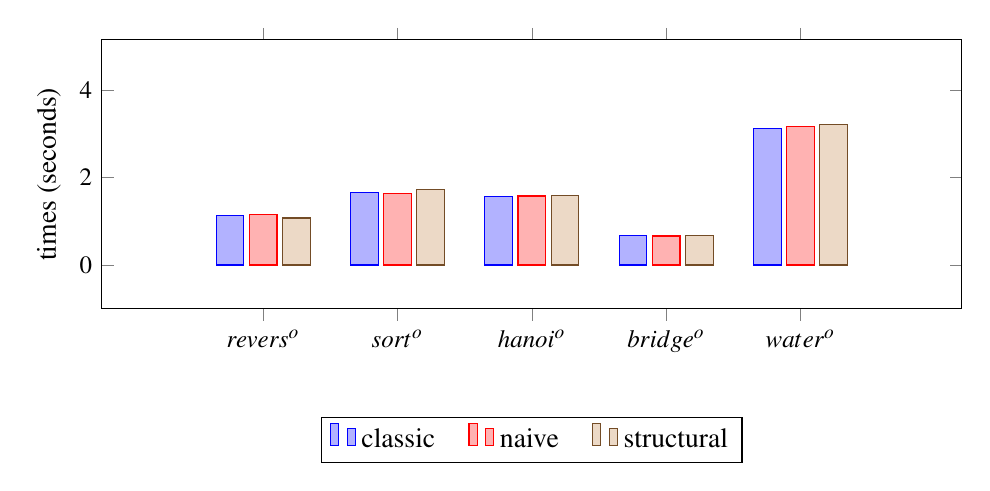
\begin{tikzpicture}
\begin{axis}[
    ybar, ymax = 4, ymin = 0.15,
    enlargelimits=0.3,
    width=125mm, height=5cm,
    legend style={at={(0.5,-0.4)},
      anchor=north,legend columns=-1},
    ylabel={times (seconds)},
    tick label style={font=\small},
    symbolic x coords={$revers^o$, $sort^o$, $hanoi^o$, $bridge^o$, $water^o$},
    xtick=data
    ]
\addplot coordinates {($revers^o$,1.142) ($sort^o$,1.664) ($hanoi^o$,1.574) ($bridge^o$,0.669) ($water^o$,3.132)};
\addplot coordinates {($revers^o$,1.151) ($sort^o$,1.636) ($hanoi^o$,1.579) ($bridge^o$,0.663) ($water^o$,3.168)};
\addplot coordinates {($revers^o$,1.077) ($sort^o$,1.723) ($hanoi^o$,1.585) ($bridge^o$,0.675) ($water^o$,3.220)};
\legend{classic$\quad$,naive$\quad$,structural}
\end{axis}
\end{tikzpicture}
\end{frame}

\begin{frame}[fragile]{Evaluation: Pessimistic Case}
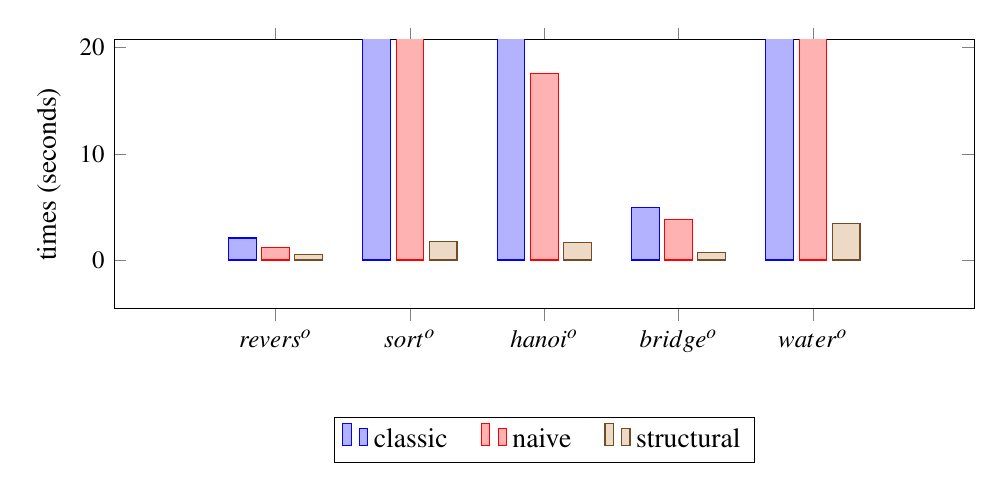
\begin{tikzpicture}
\begin{axis}[
    ybar, ymax = 16, ymin = 0.15,
    enlargelimits=0.3,
    width=125mm, height=5cm,
    legend style={at={(0.5,-0.4)},
      anchor=north,legend columns=-1},
    ylabel={times (seconds)},
    tick label style={font=\small},
    symbolic x coords={$revers^o$, $sort^o$, $hanoi^o$, $bridge^o$, $water^o$},
    xtick=data
    ]
\addplot coordinates {($revers^o$,2.073) ($sort^o$,300) ($hanoi^o$,300) ($bridge^o$,4.956) ($water^o$,300)};
\addplot coordinates {($revers^o$,1.151) ($sort^o$,300) ($hanoi^o$,17.604) ($bridge^o$,3.820) ($water^o$,300)};
\addplot coordinates {($revers^o$,0.542) ($sort^o$,1.751) ($hanoi^o$,1.646) ($bridge^o$,0.712) ($water^o$,3.414)};
\legend{classic$\quad$,naive$\quad$,structural}
\end{axis}
\end{tikzpicture}
\end{frame}

\begin{frame}[fragile]{Conclusions}
\begin{itemize}
     \item[$\bullet$] Another one formal semantics for \mk with directed conjunction
    \vskip5mm
    \item[$\bullet$] Two formal semantics for \mk with fair conjunction
    \vskip5mm
    \item[$\bullet$] Evaluation of all three semantics
\end{itemize}
\end{frame}

\begin{frame}[fragile]{Future Work}
\begin{itemize}
    \item[$\bullet$] Generalize our approach to larger class of programs
    \vskip5mm
    \item[$\bullet$] Formalize our approach in Coq proof assistant
    \vskip5mm
    \item[$\bullet$] Formally prove equivalence with denotational semantics
    \vskip5mm
    \item[$\bullet$] Formally prove conjunction fairness 
\end{itemize}
\end{frame}



\begin{frame}
\begin{center}
{\Huge Thanks!}
\end{center}
\end{frame}

\end{document}